\RequirePackage{atbegshi}
\documentclass{beamer}

%\usepackage{beamerarticle}

\usepackage{beamerthemesplit}
\usepackage{graphicx}
\usepackage{xypic}

\title{A Radio Relay System for Remote Sensors in the Antarctic}
\subtitle{Proposal Seminar}
\author{Mark Jessop}
\date{March 19, 2010}



\begin{document}

\frame{
\titlepage
\begin{center}
\small{Supervisor: Dr Chris Coleman \hspace{20pt} Co-Supervisor: Dr  Said Al-Sarawi}
\end{center}
}

%\section[Outline]{}
%\frame{\tableofcontents}

\section{Introduction}
\subsection{Project Background}
\frame
{
  \frametitle{Project Background}
  \begin{itemize}
  \item Research team operating ionospheric measurement equipment in Antarctica. 
  \item Equipment left in the field for many months at a time.
  \item Results are obtained only when the equipment is retrieved.
  \item Not much can be accomplished while the equipment is in the field.
  \item Need some way to gain access to the data!
  \end{itemize}
}
\subsection{Project Aim}
\frame{
\frametitle{Project Aim}
\begin{itemize}
\item Design and build a low power short wave data transmitter that can translate low rate data into a modulated short wave output with sufficient power to transmit the data over several hundred kilometres on an Antarctic communication path.
\end{itemize}
}

\frame{
\frametitle{Block Overview}
\begin{figure}
\xymatrix{
*++[F]{\hbox{Sensors}} \ar@{=}[dd]_{\hbox{\tiny{Data Bus}}} & \\
& *++[F]{\hbox{Buffer}} \ar[d]\\
*++[F]\hbox{{Data\ Tap}} \ar@{=>}[d] \ar[r] & *++[F]{\hbox{CPU}} \ar[u] \ar[r] & *++[F]{\txt{RF\ Signal\\Generator}} \ar[r] & *++[F]{\txt{Power\\Amp}} \ar[r] & \txt{Antenna}\\
*++[F]{Storage}&\\
}
\end{figure}
}

\section{Limitations \& Challenges}
\frame{
\frametitle{Limitations \& Challenges}
\begin{itemize}
\item Low power budget
\item Extremely cold temperatures
\item Ionospheric absorption loss
\end{itemize}
\begin{figure}
\begin{center}
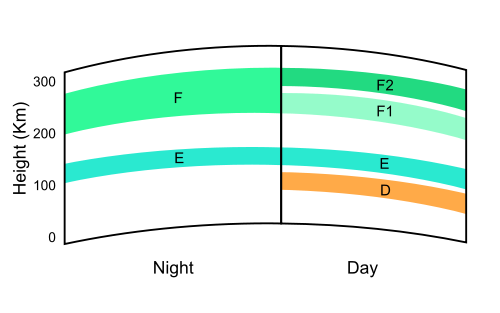
\includegraphics[height=4cm]{./images/ionosphere_500px.png}
\end{center}
\caption{Layers of the Ionosphere}
\end{figure}
}
\subsection{Power Budget}
\frame{
\frametitle{Power Budget}
\begin{itemize}
\item Equipment operates from battery power for many months at a time.
\item Efficiency is extremely important.
\item Components will need to be carefully selected for minimal power consumption.
\item Transmission frequency may need to be lowered to keep within constraints.
\end{itemize}
}
\subsection{Preliminary Sizing Calculations}
\frame{
\frametitle{Preliminary Sizing Calculations}
If we make a few assumptions, we can use the Friis transmission equation and the Shannon-Hartley Theorem to calculate the theoretical maximum bit rate of a radio link.

Assume:
\begin{itemize}
\item 200km Distance between TX and RX (on ground)
\item 400km radio path (via near-vertical skywave)
\item 5MHz Transmission frequency ($\lambda$ = 60m)
\item No ionospheric absorption loss (Not Realistic!)
\item Dipole antennas one each end ($G_t = G_r = 1.5$)
\item 10dB SNR required
\item -114dB$^{[2]}$ background noise at 5MHz
\end{itemize}
}
\frame{
\frametitle{Preliminary Sizing Calculations - SNR}
Using 1W transmission power, we can calculate the power at the receiving antenna:
\begin{flalign*}
P_r &= \frac{P_t G_t G_r}{(4\pi R /\lambda)^2}\\
&= \frac{1 \times 1.5 \times 1.5}{(4\pi \times 400000 / 60)^2} = 0.3206 nW = -94.94 dB\\
SNR &= 114 - 94.94 = 19.06dB = 80.54\\
\end{flalign*}
}

\frame{
\frametitle{Preliminary Sizing Calculations - Capacity}
We can use the Shannon-Hartley theorem to calculate the theoretical maximum channel capacity of the link:
\[C = B \log_2 (1 + SNR) \]
Where $C$ is the channel capacity (in bits/s) and B is the signal bandwidth. Assuming Binary FSK modulation is used with a 600Hz frequency shift, we calculate the maximum channel capacity as:
\[C = 600 \log_2 (1 + 80.54) = 3809.66 \mbox{ bits/s}\]

To ensure reliability, a much lower bit-rate ($\sim 600$ bits/s) would be used.
}

\frame{
\frametitle{Preliminary Sizing Calculations - Power Usage}
To get a rough idea of the power usage, let us assume we are transmitting at 600 bit/s for one hour (263.67 kB of data).

The power usage of some devices that could be used are as follows:
\begin{itemize}
\item Microcontroller - 75mW in active mode $^{[3]}$
\item Signal Generator - 40mW when active $^{[4]}$
\item Power Amplifier - 1W (idealised)
\end{itemize}
So under these ideal conditions, the transmitter will draw 1.115W when transmitting, which is 4014 Joules of energy for one hour of transmission. 

}

\subsection{Temperature}
\frame{
\frametitle{Temperature}
\begin{itemize}
\item Mean annual temperature for Antarctica's interior is $-57^\circ$C.
\item Standard industry specification is $-55^\circ$C to $+125^\circ$C. 
\item Not all devices conform to this spec, and many will be unreliable at these limits!
\end{itemize}
\begin{figure}
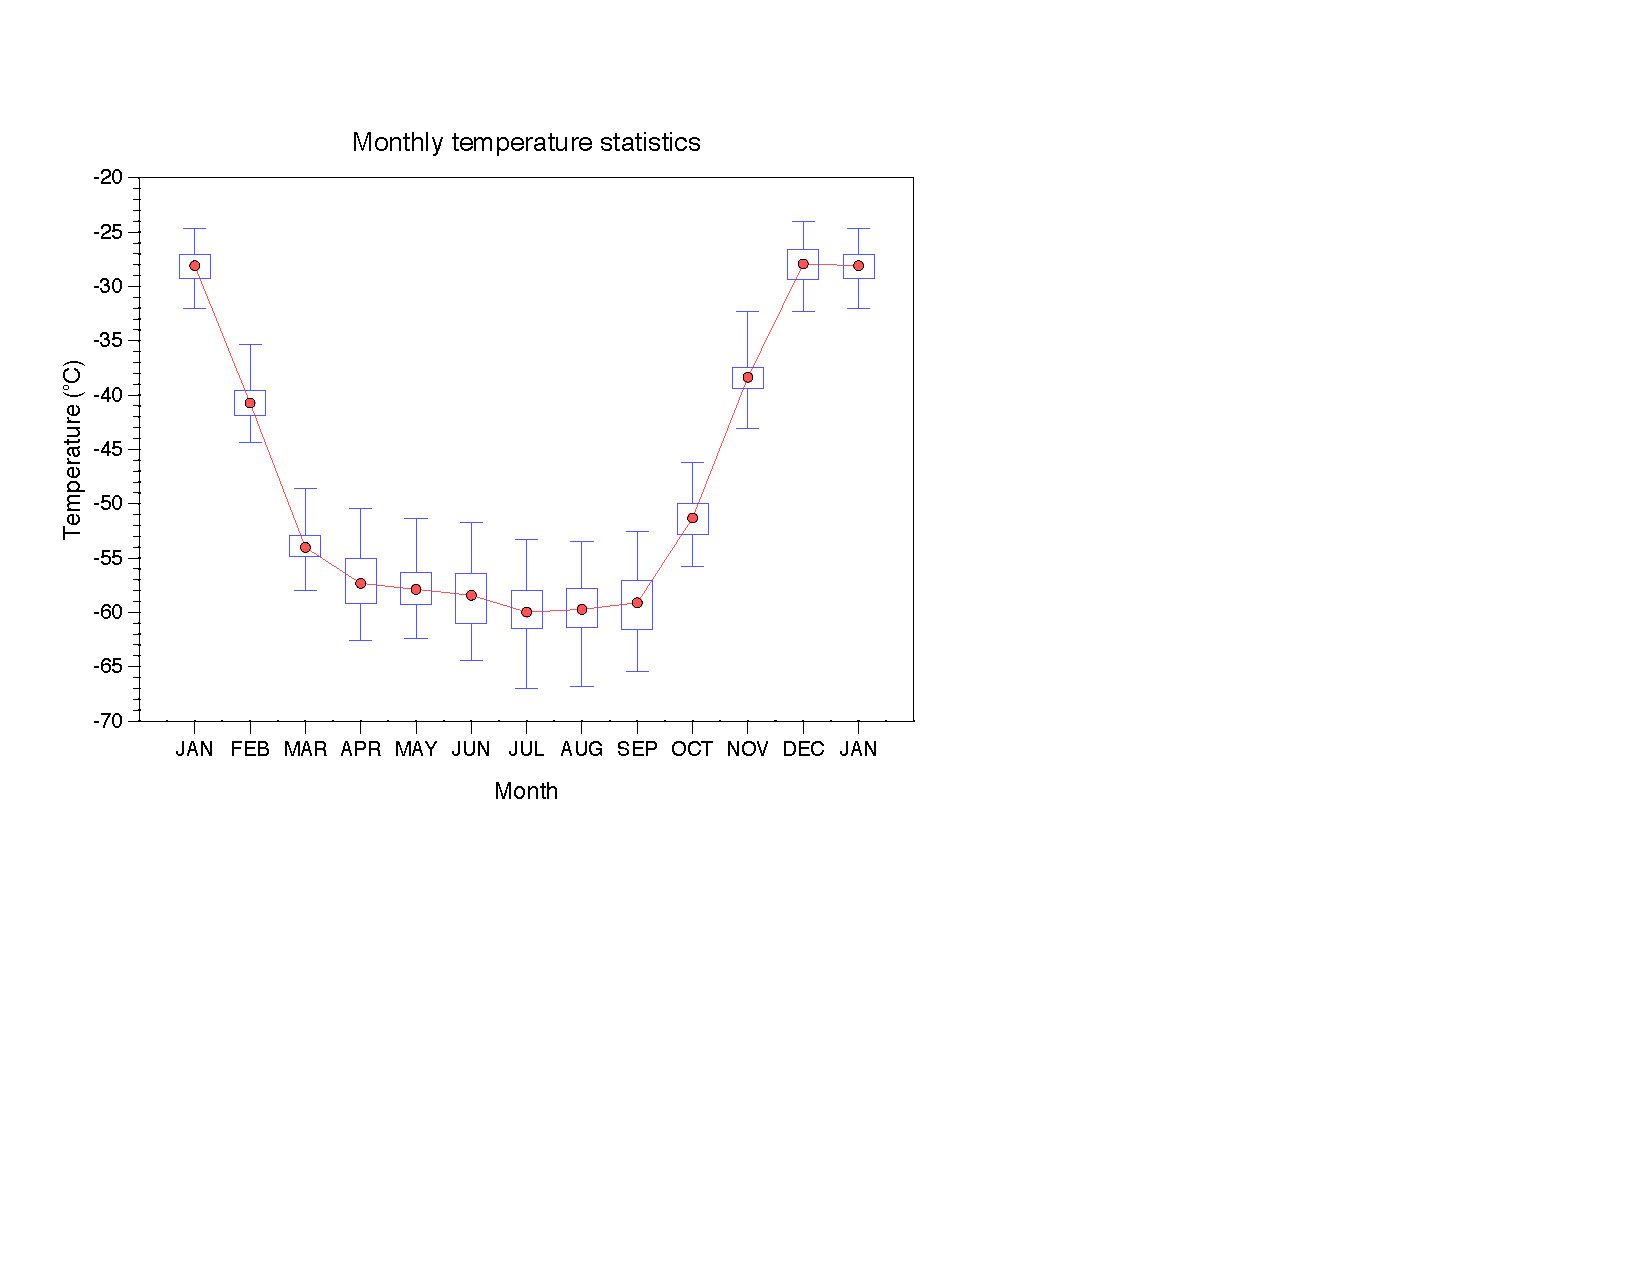
\includegraphics[height=3cm]{./images/amundsen-scott_temp_stats.pdf}
\caption{Monthly Temperature Statistics for the Amundsen Scott Research Station $^{[1]}$}
\end{figure}
}

\section{Project Plan}
%\subsection{Overview}

%\subsection{Possible Implementation Strategies}
%\frame{
%\frametitle{Possible Implementation Strategies}
%\begin{itemize}
%\item Microcontroller based (AVR, ARM, PIC)
%\item Raw Logic
%\item CPLD/FPGA
%\end{itemize}
%}

\subsection{Budget}
\frame{
\frametitle{Budget}
Maximum cost = \$250
\begin{itemize}
\item Devices for stress testing (i.e. micro-controllers) - \$50
\item RF System - \$50
\item Control System - \$50
\item PCB Construction - \$50
\end{itemize}

}

\subsection{Timeline}
\frame{
\frametitle{Timeline}
\begin{tabular}{l|l}
\textbf{Task} & \textbf{Expected Completion}\\
\hline
Background Research & S1 Week 3\\
Simulation \& Component Research & S1 Week 5\\
High-level design & S1 Week 7\\
Software Design \& Coding & End of S1\\
Hardware Design& End of S1\\
\hspace{10pt} Data-Tap &\\
\hspace{10pt} Controller &\\
\hspace{10pt} RF System &\\

Prototype construction & Early S2\\
Testing \& Optimisation & Mid S2 \\
\end{tabular}
}
\subsection{Deliverables}
\frame{
\frametitle{Deliverables}
\begin{itemize}
\item Proposal Seminar (Now!)
\item Stage 1 Design Document (S1 Week 5)
\item Progress report (S1 Week 11)
\item Interim Performance Report (S1 Week 12)
\item Final Seminar (S2 Mid-semester break)
\item Final Report (S2 Week 11)
\item Final Performance Report (S2 Week 12)
\item Project Exhibition (S2 Week 12)
\end{itemize}
}

\subsection{Risks \& Dependencies}
\frame{
\frametitle{Risks \& Dependencies}
\begin{itemize}
\item No life-threatening risks involved with this project.
\item Minor risks involving electrical/RF safety.
\item Minor risks involving hardware damage, shipping problems, etc.
\item Medium-level risk involved if project leader becomes ill.
\end{itemize}
}

\section*{References}
\frame{
\frametitle{References}
\tiny{
[1] G. Marshall. ``Monthly mean surface temperature at Amundsen-Scott station" \textit{http://www.nerc-bas.ac.uk/icd/gjma/pole.temps.html} Mar. 9, 2010 [Mar. 11, 2010]

[2] S.K. Datta. ``Radio Noise Measurement in HF/VHF Band at Antarctica" \textit{http://dspace.ncaor.org:8080/dspace/bitstream/123456789/707/1/115-119.pdf} (Google Cache), 1995 [Mar. 15, 2010]

[3] Atmel, ``ATMega168PA Electrical Characteristics", ATMega168PA Datasheet, Dec. 2009

[4] Analog Devices, ``AD9834 Specifications", AD9834 Datasheet, Feb. 2003
}
}

\section*{Q \& A}
\frame{
\frametitle{Questions \& Answers}

\LARGE{Any Questions?}
}
\end{document}